\chapter{Specifikacija programske potpore}
	
	\section{Funkcionalni zahtjevi}
			
			\noindent \textbf{Dionici:}
			
			\begin{packed_enum}
				
				\item Administrator-voditelj tima
				\item Razvojni tim CodeCooks			
				\item Profesori predmeta Programsko inženjerstvo
				\item Korisnici
				
			\end{packed_enum}
			
			\noindent \textbf{Aktori i njihovi funkcionalni zahtjevi:}
			
			
			\begin{packed_enum}
				\item  \underbar{Admin može:}
				
				\begin{packed_enum}
					
					\item Upravljanje korisnicima
					\item Upravljanje receptima
					\begin{packed_enum}
						
						\item  Brisanje recepata
						\item  Uređivanje recepata
						
					\end{packed_enum}
					\item Upravljanje komentarima
					\begin{packed_enum}
						
						\item  Brisanje komentara 
						\item  Cenzuriranje komentara
						
					\end{packed_enum}
					\item  Mijenjanje kategorija
					
				\end{packed_enum}
				
				\item  \underbar{Registrirani korisnik može:}
				
				\begin{packed_enum}
					
					\item Objavljivanje recepata
					\item Komuniciranje s ostalim registriranim korisnicima
					\item Objavljivanje termina za komunikaciju
					\item Označavanje recepata
					\item Komentiranje recepata
					\item Spremanje recepata
					\item Praćenje drugih registriranih korisnika
					\item Upravljanje dozvolama pratiteljima
					\item Upravljanje osobnim informacijama
					\item Upravljanje postavkama komunikacije i obavijestima
					
				\end{packed_enum}
				
				\item  \underbar{Neregistrirani korisnik može:}
				
				\begin{packed_enum}
					
					\item Pregledavanje recepata temeljem kategorija
					\item Pregledavanje recepata na početnoj stranici platforme
					
				\end{packed_enum}
				
				
				\item  \underbar{Baza podataka može:}
				
				\begin{packed_enum}
					
					\item Pohrana osobnih podataka registriranog korisnika
					\item Pohrana podataka o pratiteljima i pratiocima korisnika
					\item Pohrana recepata
					\item Pohrana komentara
					
				\end{packed_enum}
			\end{packed_enum}
			
			\eject 
				
			\subsection{Obrasci uporabe}
				
				
						\noindent \underbar{\textbf{UC1 - Pregled recepata}}
					\begin{packed_item}
						
						\item \textbf{Glavni sudionik: Neregistriran korisnik, Registriran korisnik}
						\item  \textbf{Cilj: Pregled recepata} 
						\item  \textbf{Sudionici: Baza podataka} 
						\item  \textbf{Preduvjet: -} 
						\item  \textbf{Opis osnovnog tijeka:}
						
						\item[] \begin{packed_enum}
							
							\item Korisnik pristupi platformi
							\item S baze podataka se na platformu dohvaća popis recepata, kategorija, vrsta kuhinje i sastojaka
							\item Korisnik može odabrati na koji način želi pregledati recepte i ovisno o tome se oni učitavaju na platformi
						\end{packed_enum}
						
					\end{packed_item}
					
					
				\noindent \underbar{\textbf{UC2 - Registracija}}
				\begin{packed_item}
					
					\item \textbf{Glavni sudionik: Neregistrirani korisnik}
					\item  \textbf{Cilj: Stvaranje računa za pristup ostalim značajkama sustava}  
					\item  \textbf{Sudionici: Baza podataka} 
					\item  \textbf{Preduvjet:-} 
					\item  \textbf{Opis osnovnog tijeka:}
					
					\item[] \begin{packed_enum}
						
						\item Korisnik odabire opciju za registraciju
						\item Korisnik unosi potrebne korisničke podatke i odabire unos
						\item Podaci se šalju sustavu i on provjerava jesu li uneseni svi potrebni podaci i postoji li već korisnik s istim imenom
						\item Ako je sve u redu sustav sprema novog korisnika u bazu podataka i šalje povratnu obavijest o registraciji 
						\item Korisnik je automatski nakon registracije prijavljen u sustav i može pregledati ostale značajke sustava
					\end{packed_enum}
					
					\item  \textbf{Opis mogućih odstupanja:}
					
					\item[] \begin{packed_item}
						
						\item[2.a] Odabir već zauzetog korisničkog imena i/ili e-maila, unos korisničkog podatka u nedozvoljenom formatu ili pružanje neispravnoga e-maila
						\item[] \begin{packed_enum}
							
							\item  Sustav obavještava korisnika o neuspjelom upisu i vraća ga na stranicu za registraciju
							\item Korisnik mijenja potrebne podatke te završava unos ili odustaje od registracije
							
						\end{packed_enum}
						
					\end{packed_item}
				\end{packed_item}
				
				
				\noindent \underbar{\textbf{UC3 - Prijava u sustav}}
				\begin{packed_item}
					
					\item \textbf{Glavni sudionik: Registrirani korisnik}
					\item  \textbf{Cilj: Omogućiti pristup ostali funkcijama sustava za korisnika} 
					\item  \textbf{Sudionici: Baza podataka} 
					\item  \textbf{Preduvjet: Registracija} 
					\item  \textbf{Opis osnovnog tijeka: }
					
					\item[] \begin{packed_enum}
						\item Korisnik odabire opciju za prijavu u sustav
						\item Na stranici za prijavu unosi korisničkog ime i lozinku i pritisne gumb za prijavu
						\item Podaci za prijavu šalju se sustavu i on provjera postoji li korisnik u bazi podataka koji ima isto korisničko ime i lozinku 
						\item Ako je sve u redu korisniku se šalje potvrda o ispravnosti unesenih podataka i prijavljen je u sustav
						\item Nakon toga može pristupiti ostalim funkcijama sustava
						
					\end{packed_enum}
					
					\item  \textbf{Opis mogućih odstupanja:}
					
					\item[] \begin{packed_item}
						
						\item[2.a] Neispravno korisničko ime/lozinka
						\item[] \begin{packed_enum}
							
							\item  Sustav obavještava korisnika o neuspjelom upisu i vraća ga na stranicu za prijavu
							
							
						\end{packed_enum}
						
						
					\end{packed_item}
				\end{packed_item}
				
				
				
				\noindent \underbar{\textbf{UC4 - Objava recepata}}
				\begin{packed_item}
					
					\item \textbf{Glavni sudionik: Registrirani korisnik }
					\item  \textbf{Cilj: Objava vlastitog recepta na sustav} 
					\item  \textbf{Sudionici: Baza podataka} 
					\item  \textbf{Preduvjet: Korisnik je prijavljen} 
					\item  \textbf{Opis osnovnog tijeka:}
					
					\item[] \begin{packed_enum}
						
						\item Korisnik odabire opciju za stvaranje novog recepta
						\item Na stranici za stvaranje recepta ispunjava formu gdje treba navesti naslov, sastojke, korake pripreme i vrijeme kuhanja
						\item Opcionalno može dodati oznake poput „vegetarijansko“, „bezglutensko“ i sl.
						\item Opcionalno može dodati slike i videozapise koji se odnose na pripremu jela
						\item Korisnik odabire objavu recepta
						\item Podaci se šalju sustav i on provjerava jesu li svi podatci u redu, ako jesu recept se sprema u bazu podataka 
						\item Korisnik prima obavijest da je uspješno objavio recept i može ga ići pregledati
						
					\end{packed_enum}
					
					\item  \textbf{Opis mogućih odstupanja:}
					
					\item[] \begin{packed_item}
						
						\item[2.a] Korisnik nije naveo naslov, sastojke, korake pripreme i vrijeme kuhanja
						\item[] \begin{packed_enum}
							
							\item Sustav obavještava korisnika o neuspjelom upisu u bazu i vraća ga na stranicu za objavu recepata (UC4.2)
							
						\end{packed_enum}
						
					\end{packed_item}
				\end{packed_item}
				
				
				\noindent \underbar{\textbf{UC5 - Uređivanje recepata od strane korisnika}}
				\begin{packed_item}
					
					\item \textbf{Glavni sudionik: Registrirani korisnik}
					\item  \textbf{Cilj: Uređivanje svog objavljenog recepta} 
					\item  \textbf{Sudionici: Baza podataka} 
					\item  \textbf{Preduvjet: Objavljen je recept i korisnik je prijavljen} 
					\item  \textbf{Opis osnovnog tijeka:}
					
					\item[] \begin{packed_enum}
						
						\item Korisnik na stranici recepta pregledava svoj recept
						\item Korisnik može odabrati gumb za uređivanje recepta
						\item Otvori se forma gdje korisnik može uređivati recepta kao pri objavi
						\item Korisnik može odabrati spremanje recepta ili odustajanje od promjena
						\item Ako je korisnik odlučio spremiti recept podaci o ažuriranom receptu šalju se sustavu koji provjerava jesu li u redu i ako jesu sprema se u bazu podataka, a ako je korisnik odustao od promjena korisnika se vraća na stranicu recepta
					\end{packed_enum}
					
					
				\end{packed_item}
				
				\noindent \underbar{\textbf{UC6 - Brisanje recepata od strane korisnika}}
				\begin{packed_item}
					
					\item \textbf{Glavni sudionik: Registrirani korisnik}
					\item  \textbf{Cilj: Brisanje svog objavljenog recepta} 
					\item  \textbf{Sudionici: Baza podataka} 
					\item  \textbf{Preduvjet: Objavljen je recept i korisnik je prijavljen} 
					\item  \textbf{Opis osnovnog tijeka:}
					
					\item[] \begin{packed_enum}
						
						\item Korisnik na stranici recepta pregledava svoj recept
						\item Korisnik može odabrati gumb za brisanje recepta
						\item U skočnom prozoru potvrđuje ili odustaje od brisanja recepta 
						\item Ako je korisnik odlučio obrisati recept zahtjev se šalje u sustav koji obriše recept iz baze podataka, a ako je odustao vraća se na stranicu recepta
						
					\end{packed_enum}
				\end{packed_item}
				
				
				\noindent \underbar{\textbf{UC7 - Razmjena poruka}}
				\begin{packed_item}
					
					\item \textbf{Glavni sudionik: Registrirani korisnici i oni koji su objavili recept }
					\item  \textbf{Cilj: Komunikacija između korisnika u vezi recepata} 
					\item  \textbf{Sudionici: Baza podataka, Firebase} 
					\item  \textbf{Preduvjet: Korisnici su prijavljeni, autor je dostupan i ima objavljen recept} 
					\item  \textbf{Opis osnovnog tijeka:}
					
					\item[] \begin{packed_enum}
						
						\item Korisnik pregledava profil drugog korisnika gdje može odabrati gumb za početak razmjene poruka
						\item Korisniku se prikaže forma gdje može upisati predmet poruke i sadržaj poruke te ju poslati korisniku
						\item Sustav provjerava je li sve u redu s porukom i ako je ju sprema na Firebase poslužitelj preko kojega se onda poruka dostavlja drugome korisniku
						\item Drugi korisnik prima obavijest o primljenoj poruci i može ju pregledati te na nju odgovoriti
					\end{packed_enum}
				
				\end{packed_item}
				
				\noindent \underbar{\textbf{UC8 - Čavrljanje }}
				\begin{packed_item}
					
					\item  \textbf{Glavni sudionik: Registrirani korisnici i oni koji su objavili recept }
					\item  \textbf{Cilj: Komunikacija između korisnika u vezi recepata} 
					\item  \textbf{Sudionici: Baza podataka, Firebase} 
					\item  \textbf{Preduvjet: Korisnici su prijavljeni, autor je dostupan i ima objavljen recept} 
					\item  \textbf{Opis osnovnog tijeka:}
					
					\item[] \begin{packed_enum}
						
						\item Korisnik pregledava profil drugog korisnika gdje može odabrati gumb za čavrljanje 
						\item Ovaj zahtjev se pohranjuje na Firebase poslužitelj i šalje se zahtjev za čavrljanje drugom korisniku
						\item Drugi korisnik treba prihvatiti ili odbiti zahtjev za čavrljanje, ova informacija se onda pohranjuje na Firebase poslužitelj
						\item Ako je uspostavljenja komunikacija otvori se prozor za čavrljanje gdje korisnici mogu razmjenjivati poruke
						
					\end{packed_enum}
					
					\item  \textbf{Opis mogućih odstupanja:}
					
					\item[] \begin{packed_item}
						
						\item[2.a] Autor nije dostupan u to doba za čavrljanje
						\item[] \begin{packed_enum}
							
							\item Korisnika obavještavamo da autor nije dostupan i vraćamo ga na pregled recepta
							
						\end{packed_enum}
						
					\end{packed_item}
				\end{packed_item}
				
				\noindent \underbar{\textbf{UC9 - Video poziv}}
				\begin{packed_item}
					
					\item \textbf{Glavni sudionik: Registrirani korisnici i oni koji su objavili recept }
					\item  \textbf{Cilj: Komunikacija između korisnika u vezi recepata} 
					\item  \textbf{Sudionici: Baza podataka, Firebase} 
					\item  \textbf{Preduvjet: Korisnici su prijavljeni, autor je dostupan i ima objavljen recept} 
					\item  \textbf{Opis osnovnog tijeka:}
					
					\item[] \begin{packed_enum}
						
						\item Korisnik pregledava profil drugog korisnika gdje može odabrati gumb za video poziv
						\item Zahtjev se sprema na Firebase poslužitelj i šalje drugom korisniku
						\item Drugi korisnik prima zahtjev za videopozivom i može prihvatiti ili odbiti poziv
						\item Ako je poziv prihvaćen traje sve dok ga jedan od korisnika ne prekine
					\end{packed_enum}
					
					\item  \textbf{Opis mogućih odstupanja:}
					
					\item[] \begin{packed_item}
						
						\item[2.a] Autor nije dostupan u to doba za videopoziv
						\item[] \begin{packed_enum}
							
							\item Korisnika obavještavamo da autor nije dostupan i vraćamo ga na pregled recepta
							
						\end{packed_enum}
						
					\end{packed_item}
				\end{packed_item}
				
				
				
				\noindent \underbar{\textbf{UC10 - Označavanje recepata}}
				\begin{packed_item}
					
					\item \textbf{Glavni sudionik: Registrirani korisnik}
					\item  \textbf{Cilj: Označavanje da nam se recept svidio} 
					\item  \textbf{Sudionici: Baza podataka} 
					\item  \textbf{Preduvjet: Korisnik je prijavljen} 
					\item  \textbf{Opis osnovnog tijeka:}
					
					\item[] \begin{packed_enum}
						
						\item Korisnik pregledava stranicu recept i može stisnuti gumb kako bi označio da mu se recept svidio
						\item Kada korisnik pritisne gumb sustav ovu informaciju šalje u bazu podataka i poveća se broj oznaka za pregledani recept
					\end{packed_enum}
					
					
				\end{packed_item}
				
				
				\noindent \underbar{\textbf{UC11 - Komentiranje recepata}}
				\begin{packed_item}
					
					\item \textbf{Glavni sudionik: Registrirani korisnik}
					\item  \textbf{Cilj: Postavljanje komentara na recept} 
					\item  \textbf{Sudionici: Baza podataka} 
					\item  \textbf{Preduvjet: Korisnik je prijavljen i postoji recept} 
					\item  \textbf{Opis osnovnog tijeka:}
					
					\item[] \begin{packed_enum}
						
						\item Korisnik pregledava stranicu za recept gdje na dnu stranice postoji prostor gdje se prikazuju komentari, a uz njih i forma gdje korisnik može dodati svoj novi komentar
						\item Kada korisnik ispuni formu podaci se šalju sustavu i ako su u redu pohranjuju se u bazu podataka te nakon toga prikazuju na stranici recepta
					\end{packed_enum}
					
					\item  \textbf{Opis mogućih odstupanja:}
					
					\item[] \begin{packed_item}
						
						\item[2.a] Prekršili smo ograničenje na broju znakova u komentaru
						\item[] \begin{packed_enum}
							
							\item Obavještavamo korisnika o maksimalnom broju znakova i ne dopuštamo mu objaviti komentar 
						\end{packed_enum}
						
						
					\end{packed_item}
				\end{packed_item}
				
				
				\noindent \underbar{\textbf{UC12 - Spremanje recepata za buduću referencu}}
				\begin{packed_item}
					
					\item  \textbf{Glavni sudionik: Registrirani korisnik}
					\item  \textbf{Cilj: Spremanje recepta da ga korisnik može ponovno lako pronaći} 
					\item  \textbf{Sudionici: Baza podataka} 
					\item  \textbf{Preduvjet: Korisnik je prijavljen i postoji recept} 
					\item  \textbf{Opis osnovnog tijeka:}
					
					\item[] \begin{packed_enum}
						
						\item Korisnik pregledava stranicu recepta i može odabrati gumb za spremanje recepta
						\item Ako korisnik ovo odabere ova informacija se šalje sustavu koji je onda pohranjuje u bazu podataka
						\item Ako je spremanje uspješno korisnik može pregledati svoje spremljene recepte na zasebnoj stranici
					\end{packed_enum}
				\end{packed_item}
				
				
				\noindent \underbar{\textbf{UC13 - Uklanjanje oznake recepata}}
				\begin{packed_item}
					
					\item \textbf{Glavni sudionik: Registrirani korisnik}
					\item  \textbf{Cilj: Uklanjanje recepta iz favorita} 
					\item  \textbf{Sudionici: Baza podataka} 
					\item  \textbf{Preduvjet: Korisnik je prijavljen} 
					\item  \textbf{Opis osnovnog tijeka:}
					
					\item[] \begin{packed_enum}
						
						\item Korisnik pregledava stranicu recepta kojeg je već označio
						\item Korisnik oznaku može ukloniti ponovnim pritiskom na gumb za označavanje recepta
						\item Ako korisnik ovo pritisne ova informacija se šalje u bazu podataka i mijenja se broj oznaka za pregledavani recept
					\end{packed_enum}
					
					
				\end{packed_item}
				
				
				\noindent \underbar{\textbf{UC14 - Uklanjanje komentara}}
				\begin{packed_item}
					
					\item \textbf{Glavni sudionik: Registrirani korisnik}
					\item  \textbf{Cilj: Postavljanje komentara na recept} 
					\item  \textbf{Sudionici: Baza podataka} 
					\item  \textbf{Preduvjet: Korisnik je prijavljen i postoji recept} 
					\item  \textbf{Opis osnovnog tijeka:}
					
					\item[] \begin{packed_enum}
						\item Korisnik pregledava stranicu za recept gdje na dnu stranice postoji prostor gdje se prikazuju komentari, a uz njih može vidjeti i svoj komentar
						\item Na svome komentaru korisnik može vidjet gumb za uklanjanje komentar i ako ga pritisne šalju se informacije sustavu da treba obrisati taj komentar
						\item Kada sustav primi ovu informaciju briše traženi komentar iz baze podataka i on se više neće prikazivati na stranici
					\end{packed_enum}
					
					
				\end{packed_item}
				
				\noindent \underbar{\textbf{UC15 - Uklanjanje spremljenog recepta}}
				\begin{packed_item}
					
					\item  \textbf{Glavni sudionik: Registrirani korisnik}
					\item  \textbf{Cilj: Spremanje recepta da ga korisnik može ponovno lako pronaći} 
					\item  \textbf{Sudionici: Baza podataka} 
					\item  \textbf{Preduvjet: Korisnik je prijavljen i postoji recept} 
					\item  \textbf{Opis osnovnog tijeka:}
					
					\item[] \begin{packed_enum}
						
					\item Korisnik pregledava stranicu recepta kojeg je već spremio
					\item Korisnik može ponovno pritisnuti gumb za spremanje recepta kako bi ga uklonio iz svojih spremljenih recepata
					\item Kada korisnik ovo pritisne sustav obrađuje ovaj zahtjev i uklanja spremljeni recept iz tablice spremljenih recepata tog korisnika u bazi podataka
					\end{packed_enum}
				\end{packed_item}
				
				
				\noindent \underbar{\textbf{UC16 - Praćenje omiljenih autora recepata}}
				\begin{packed_item}
					
					\item  \textbf{Glavni sudionik: Registrirani korisnik}
					\item  \textbf{Cilj: Praćenje omiljenih autora kako bi korisnik dobio obavijesti o novim receptima} 
					\item  \textbf{Sudionici: Baza podataka} 
					\item  \textbf{Preduvjet: Korisnik je prijavljen} 
					\item  \textbf{Opis osnovnog tijeka:}
					
					\item[] \begin{packed_enum}
						
						\item Korisnik pregledava profil drugog korisnika na kojem se nalazi gumb za praćenje profila
						\item Ako korisnik pritisne gumb sustav obrađuje taj zahtjev i pohranjuje drugog korisnika kao profil koji prvi korisnik prati u tablicu pratioca, a uz to pohranjuje i prvog korisnika u tablicu pratitelja drugog korisnika u bazi podataka
						\item Korisnik sada prati drugog korisnika
						
					\end{packed_enum}
					
				\end{packed_item}
				
				
				\noindent \underbar{\textbf{UC17 - Uklanjanje praćenja omiljenih autora recepata}}
				\begin{packed_item}
					
					\item  \textbf{Glavni sudionik: Registrirani korisnik} 
					\item  \textbf{Cilj: Uklanjanje praćenja omiljenih autora recepata} 
					\item  \textbf{Sudionici: Baza podataka} 
					\item  \textbf{Preduvjet: Korisnik je prijavljen} 
					\item  \textbf{Opis osnovnog tijeka:}
					
					\item[] \begin{packed_enum}
						
						\item Korisnik pregledava profil drugog korisnika kojeg već prati na kojem se nalazi gumb za praćenje profila 
						\item Ako korisnik ponovno pritisne gumb sustav obrađuje taj zahtjev i uklanja informacije o praćenju tog profila iz baze podataka
						\item Korisnik više ne prati drugog korisnika
						
					\end{packed_enum}
					
				\end{packed_item}
				
				
				\noindent \underbar{\textbf{UC18 - Slanje obavijesti o novim receptima omiljenih autora }}
				\begin{packed_item}
					
					\item \textbf{Glavni sudionik: Registrirani korisnik}
					\item  \textbf{Cilj: Obavještavanje korisnika o novim objavama recepata } 
					\item  \textbf{Sudionici: Baza podataka} 
					\item  \textbf{Preduvjet: Korisnik je prijavljen i prati neke autore} 
					\item  \textbf{Opis osnovnog tijeka:}
					
					\item[] \begin{packed_enum}
						
						\item U aplikaciji postoji dio za obavijest, ima ikonicu zvonca i ako ima novih obavijest pored zvonca se pojavi trenutni broj obavijest, osim toga se korisnika obavijesti i notifikacijom
						\item Kada profil kojeg korisnik prati objavi nešto novo taj profil će dohvatiti popis svojih pratitelja iz baze podataka i poslati svima obavijest da je dodan novi recept
					\end{packed_enum}
					
				\end{packed_item}
				
				\noindent \underbar{\textbf{UC19 - Pregled javnog profila}}
				\begin{packed_item}
					
					\item \textbf{Glavni sudionik: Neregistrirani korisnik, Registrirani korisnik}
					\item  \textbf{Cilj: Pregled javnog profila nekog korisnika} 
					\item  \textbf{Sudionici: Baza podataka} 
					\item  \textbf{Preduvjet: -} 
					\item  \textbf{Opis osnovnog tijeka:}
					
					\item[] \begin{packed_enum}
						
						\item Korisnik odabire profil nekog korisnika za pregled preko recepta, može odabrati i vlastiti
						\item Sustav iz baze podataka dohvaća podatke o profilu korisnika kojeg želimo pregledati i učitava ih na stranici
						\item Tamo korisnik može pregledati objavljene recepte, pratitelje i autore koje taj korisnik prati i koji prate njega
						\item Ako profil pripada korisniku na profilu će se pojaviti gumb za pristup privatnom profilu gdje korisnik može mijenjati postavke, inače će se prikazati gumbi za komunikaciju i praćenje profila
					\end{packed_enum}
					
				\end{packed_item}
				
				\noindent \underbar{\textbf{UC20 - Pregled i promjena postavki privatnog profila}}
				\begin{packed_item}
					
					\item \textbf{Glavni sudionik: Registrirani korisnik}
					\item  \textbf{Cilj: Pregled vlastitog privatnog profila} 
					\item  \textbf{Sudionici: Baza podataka} 
					\item  \textbf{Preduvjet: Prijava korisnika} 
					\item  \textbf{Opis osnovnog tijeka:}
					
					\item[] \begin{packed_enum}
						
						\item Korisnik tijekom pregleda svog profila odabira pristup privatnom profilu
						\item Sustav iz baze podataka dohvaća podatke o profilu korisnika i učita ih u formu 
						\item Tamo korisnik može pregledati osobne informacije, postavke komunikacije, obavijesti za poruke i aktivnosti povezane s receptima te izmjenjivati podatke prema želji 
						\item Nakon izmjene ih može pohraniti ili odustati od pohrane
						\item Ako ih je odlučio pohraniti podaci se šalju sustavu koji ih obrađuje i provjerava te ako je sve uredu ažurira u bazi podataka
						
					\end{packed_enum}
					
				\end{packed_item}
				
				\noindent \underbar{\textbf{UC21- Upravljanje korisnicima od strane sistemskom administratora}}
				\begin{packed_item}
					
					\item \textbf{Glavni sudionik: Sistemski administrator}
					\item  \textbf{Cilj: Upravljanje korisnicima od strane sistemskom administratora} 
					\item  \textbf{Sudionici: Baza podataka} 
					\item  \textbf{Preduvjet: Postoje registrirani korisnici} 
					\item  \textbf{Opis osnovnog tijeka:}
					
					\item[] \begin{packed_enum}
						
						\item Administrator pregledava profil nekog korisnika na kojem se nalaze gumbi za uređivanje profila korisnika te za brisanje profila korisnika 
						\item Ako administrator odabere uređivanje profila korisnika otvorila bi se forma u sličnom obliku kao i kod uređivanja privatnog profila korisnika gdje administrator može izmijeniti podatke korisnika te ih zatim pohraniti
						\item Nakon što ih pohrani sustav ih obrađuje i ažurira u bazi podataka
						\item Ako administrator odabere brisanje korisničkog profila sustav šalje zahtjev za uklanjanje profila iz baze podataka

					\end{packed_enum}
					
				\end{packed_item}
				
				\noindent \underbar{\textbf{UC22 - Mijenjanje recepata od strane sistemskih administratora}}
				\begin{packed_item}
					
					\item \textbf{Glavni sudionik: Sistemski administrator}
					\item  \textbf{Cilj: Uređivanje (kategorija) recepta nekog korisnika} 
					\item  \textbf{Sudionici: Baza podataka} 
					\item  \textbf{Preduvjet: Postoji objavljeni recept} 
					\item  \textbf{Opis osnovnog tijeka:}
					
					\item[] \begin{packed_enum}
						
						\item Sistemski administrator pregledava recept na kojem postoji gumb za uređivanje recepta
						\item Ako administrator odabere navedeni gumb otvorit će mu se forma gdje može mijenjati podatke o receptu te ih zatim pohraniti
						\item Ako ih odluči pohraniti sustav ih obrađuje i ažurira u bazi podataka
						
					\end{packed_enum}
					
				\end{packed_item}
				
				
				\noindent \underbar{\textbf{UC23 - Brisanje recepata od strane sistemskih administratora}}
				\begin{packed_item}
					
					\item \textbf{Glavni sudionik: Sistemski administrator}
					\item  \textbf{Cilj: Brisanje recepta nekog korisnika} 
					\item  \textbf{Sudionici: Baza podataka} 
					\item  \textbf{Preduvjet: Postoji objavljeni recept} 
					\item  \textbf{Opis osnovnog tijeka:}
					
					\item[] \begin{packed_enum}
						
					\item Sistemski administrator pregledava recept na kojem postoji gumb za brisanje recepta
					\item Ako administrator odabere navedeni gumb sustav će poslati zahtjev koji će ukloniti recept iz baze podataka	
					\end{packed_enum}
					
				\end{packed_item}
				
				\eject
				\subsubsection{Dijagrami obrazaca uporabe}
				
				\begin{figure}[H]
					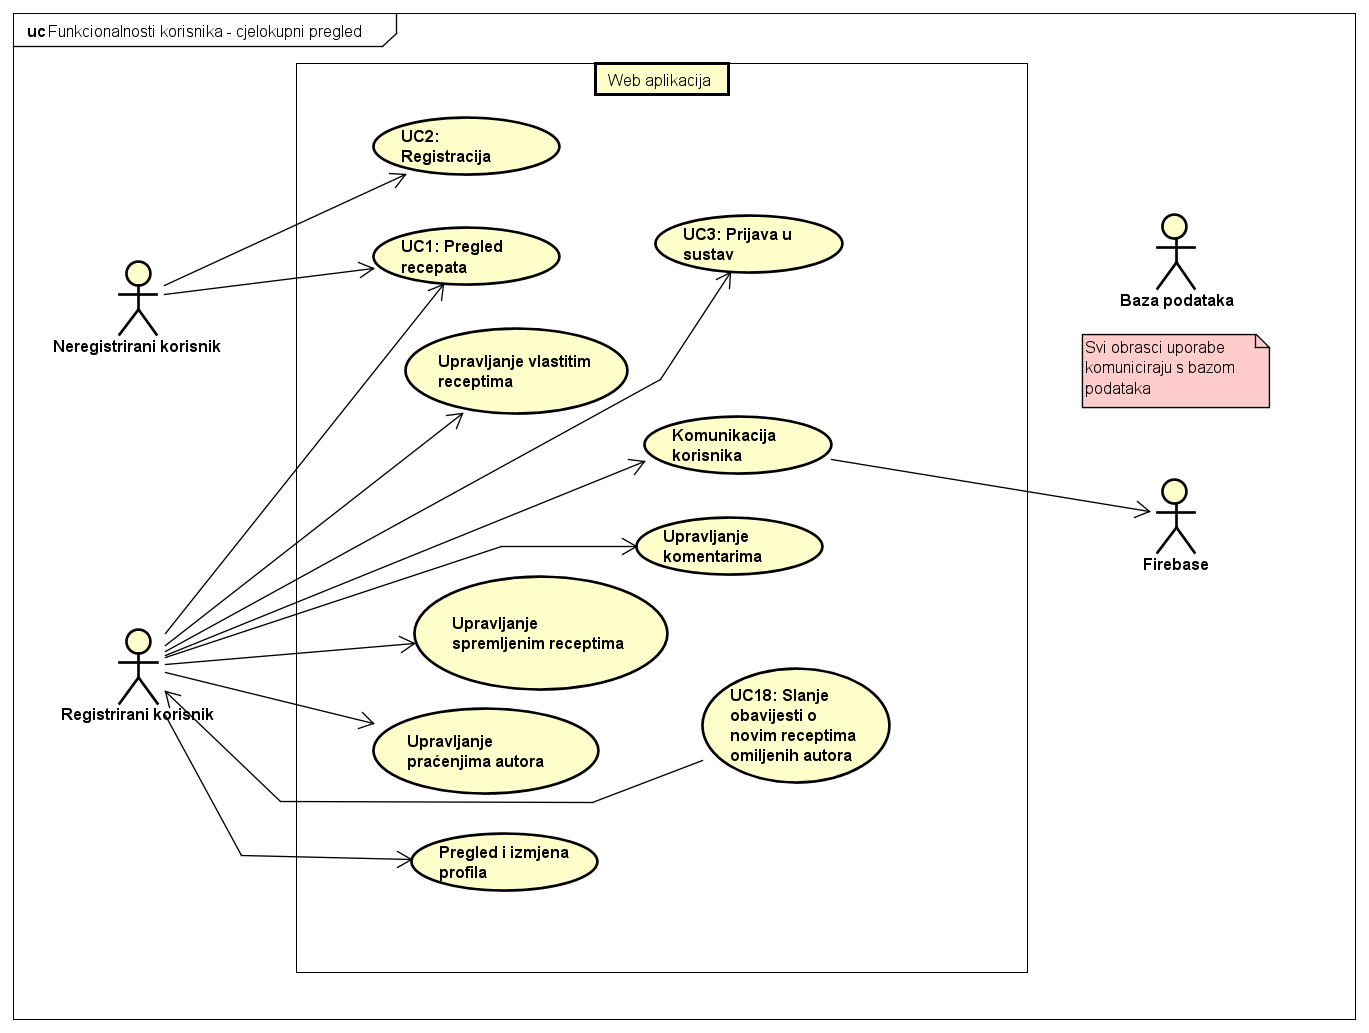
\includegraphics[scale= 0.42]{slike/UseCase Diagram0.png}
					\centering
					\caption{Dijagram obrazaca uporabe, funkcionalnosti korisnika}
					\label{fig:Dijagram obrazaca uporabe, funkcionalnosti korisnika}
				\end{figure}
				\eject
				\begin{figure}[H]
					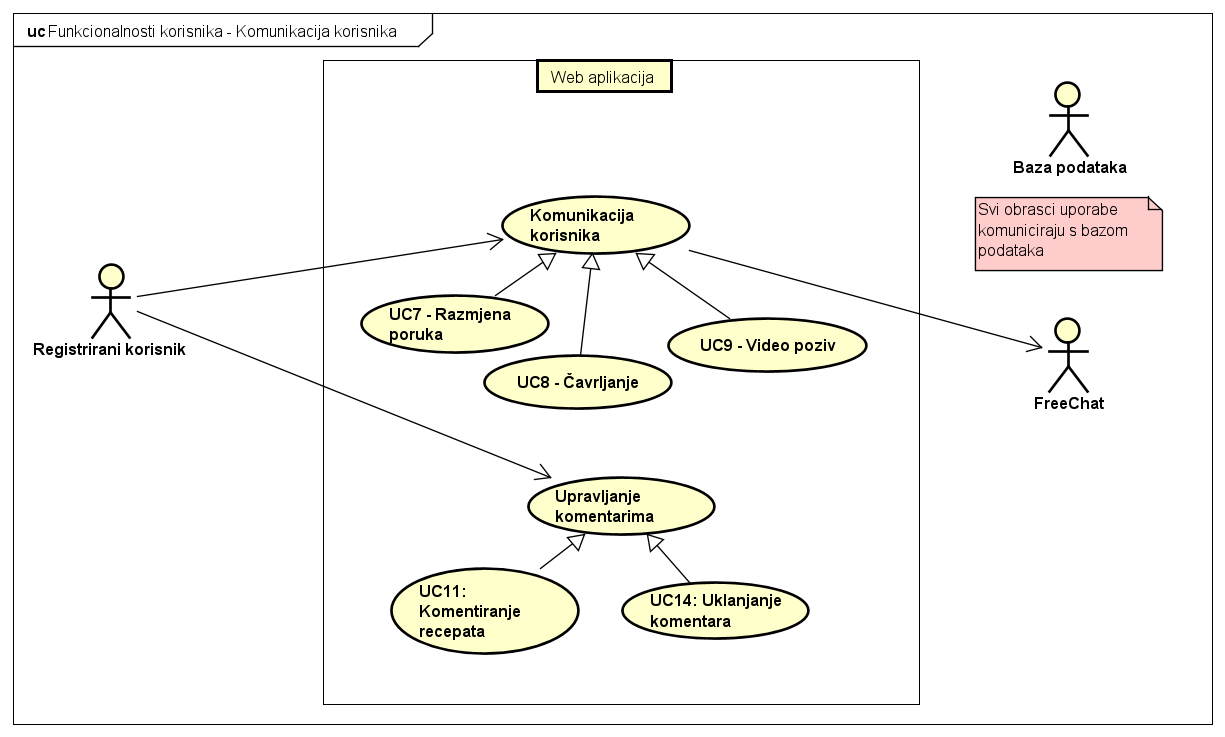
\includegraphics[scale= 0.42]{slike/UseCase Diagram1.png}
					\centering
					\caption{Dijagram obrazaca uporabe, komunikacija korisnika}
					\label{fig:Dijagram obrazaca uporabe, komunikacija korisnika}
				\end{figure}
				\begin{figure}[H]
					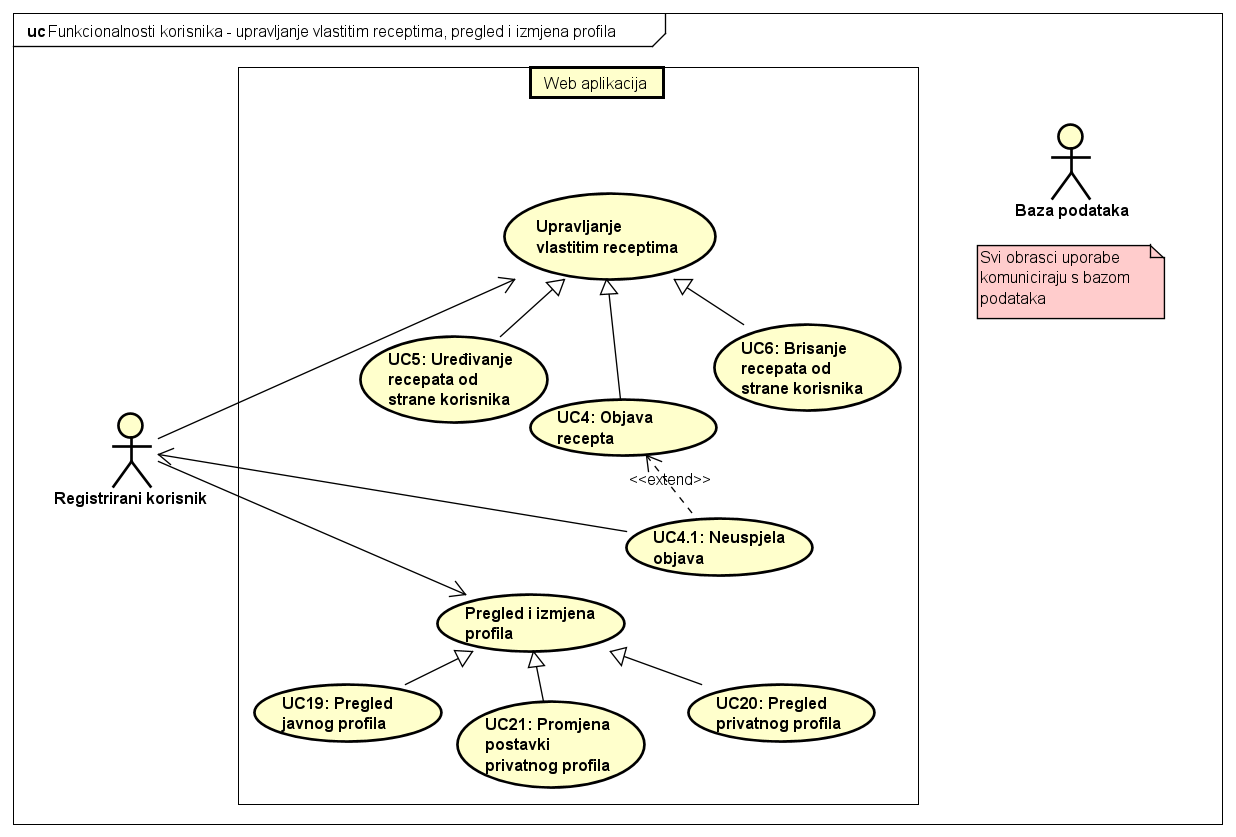
\includegraphics[scale= 0.42]{slike/UseCase Diagram2.png}
					\centering
					\caption{Dijagram obrazaca uporabe, upravljanje receptima, pregled i izmjena profila}
					\label{fig:Dijagram obrazaca uporabe, upravljanje receptima, pregled i izmjena profila}
				\end{figure}
				\begin{figure}[H]
					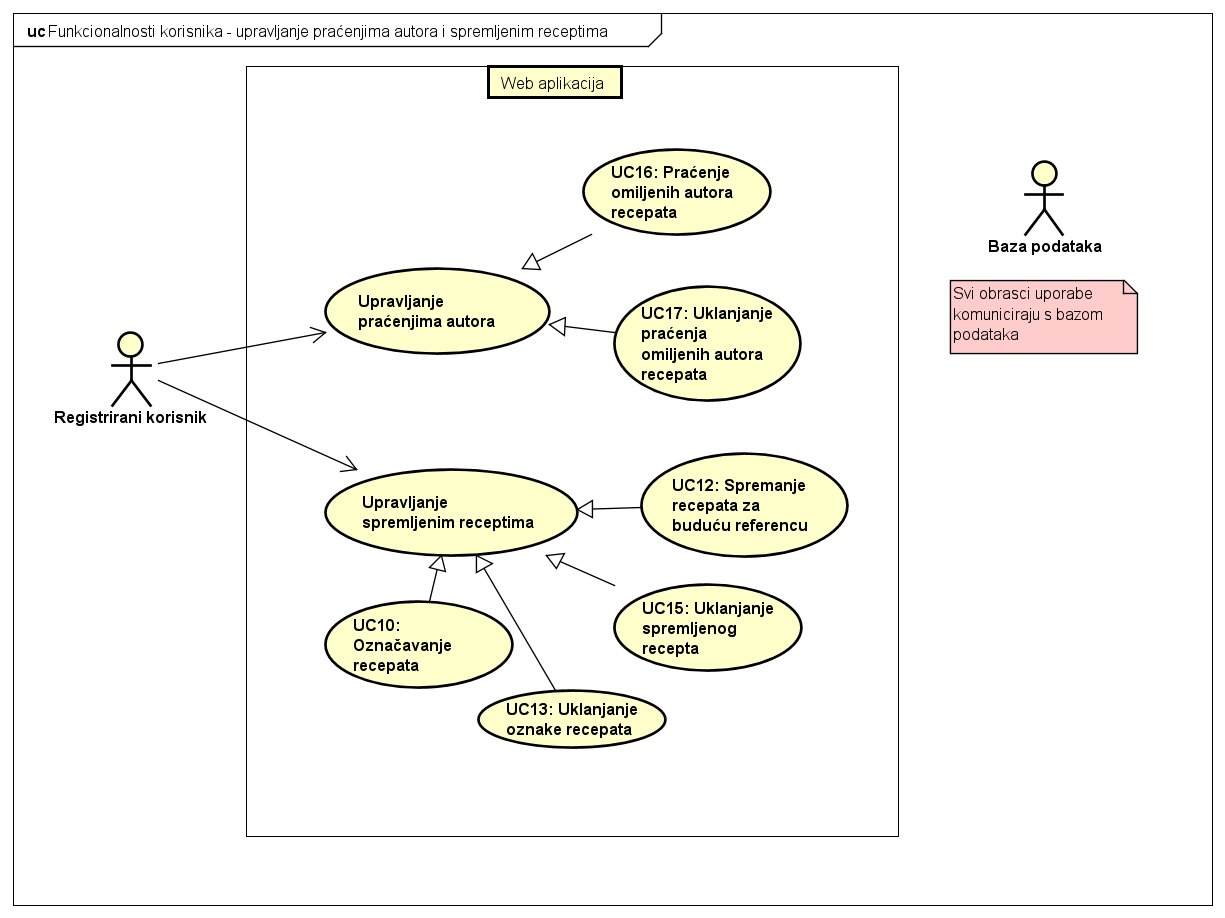
\includegraphics[scale= 0.42]{slike/UseCase Diagram3.png}
					\centering
					\caption{Dijagram obrazaca uporabe, praćenje autora i spremanje recepata}
					\label{fig:Dijagram obrazaca uporabe, praćenje autora i spremanje recepata}
				\end{figure}
				\begin{figure}[H]
					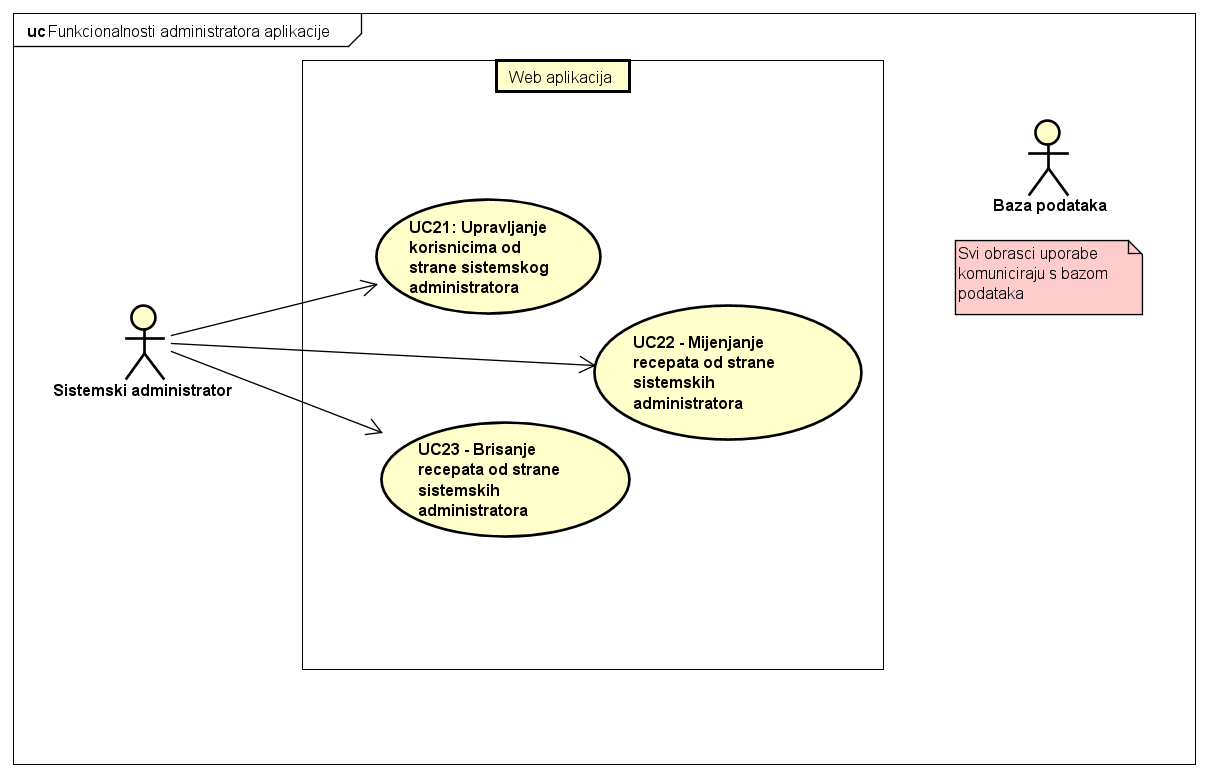
\includegraphics[scale= 0.42]{slike/UseCase Diagram4.png}
					\centering
					\caption{Dijagram obrazaca uporabe, funkcionalnosti administratora}
					\label{fig:Dijagram obrazaca uporabe, funkcionalnosti administratora}
				\end{figure}
				
				\eject		
				
				\subsection{Sekvencijski dijagrami}
				
				\noindent
				\textbf{Obrazac uporabe UC1-Pregled recepata}\newline
				{Korisnik šalje zahtjev za prikaz recepata po kategorijama, sastojcima i/ili kuhinjama kojim pripadaju. Poslužitelj dohvaća recepete koji zadovoljavaju uvjete i prikazuje ih korisniku. Korisnik sada može spremiti recepte, ako je prijavljen to se provodi, ako nije preusmjeri ga se na stranicu za prijavu.}
				
				
				\begin{figure}[H]
					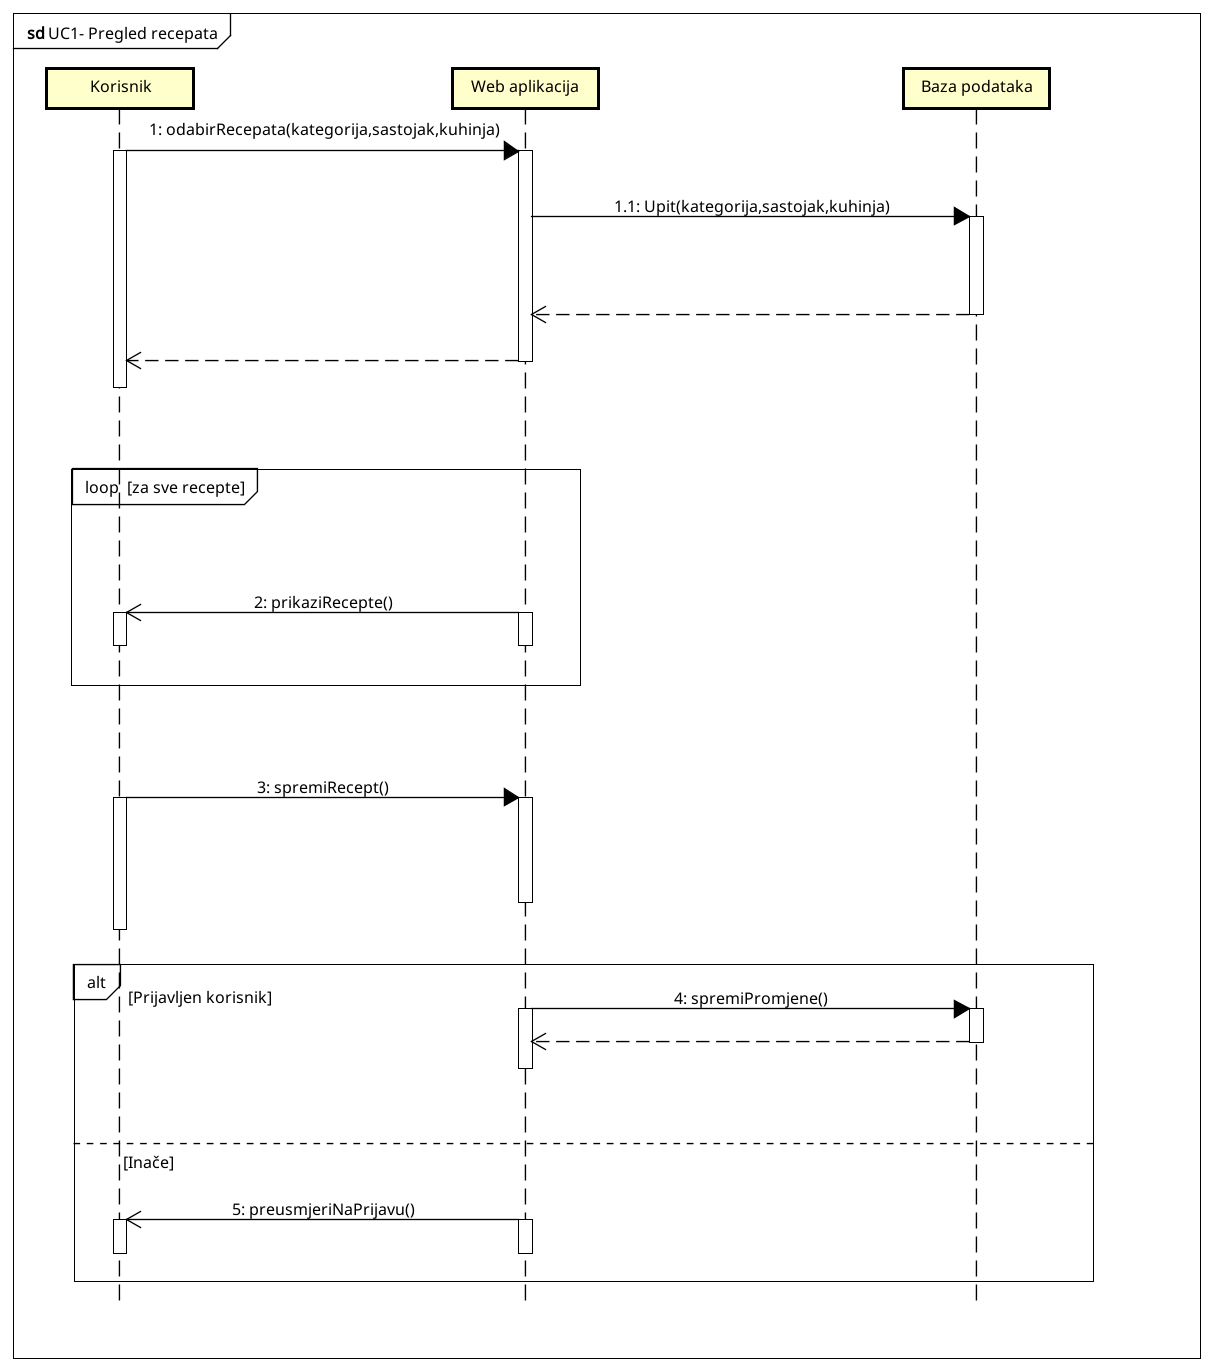
\includegraphics[scale= 0.4]{slike/sekvencijski_dijagramUC1.png}
					\centering
					\caption{Sekvencijski dijagram za UC1}
					\label{fig:Sekvencijski dijagram za UC1}
				\end{figure} 
				\eject
				
				\noindent
				\textbf{Obrazac uporabe UC3-Registracija}\newline
				{Korisnik se registrira s korisničkim imenom i lozinkom. Ako takav korisnik već postoji, korisniku se ispisuje greška. Inače, korisnik se uspješno registrirao i to se bilježi u bazi podataka.}
				
				
				\begin{figure}[H]
					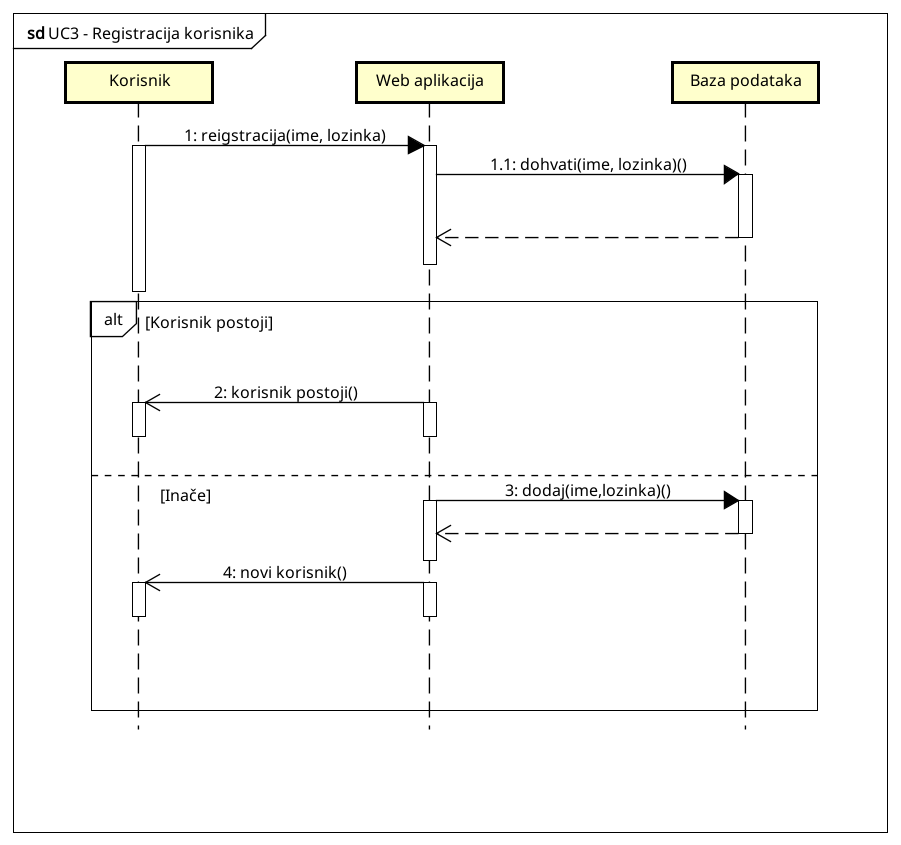
\includegraphics[scale= 0.6]{slike/sekvencijski_dijagramUC3.png}
					\centering
					\caption{Sekvencijski dijagram za UC3}
					\label{fig:Sekvencijski dijagram za UC3}
				\end{figure}
				
				\eject
				
				\noindent
				\textbf{Obrazac uporabe UC4-Prijava Korisnika}\newline
				{Korisnik pokuša objaviti novi recept. Ako nije prijavljen, preusmjeri ga se na prijavu. Inače, recept se dodaje u bazu podataka i o tome se obavijesti korisnik.}
				
				
				\begin{figure}[H]
					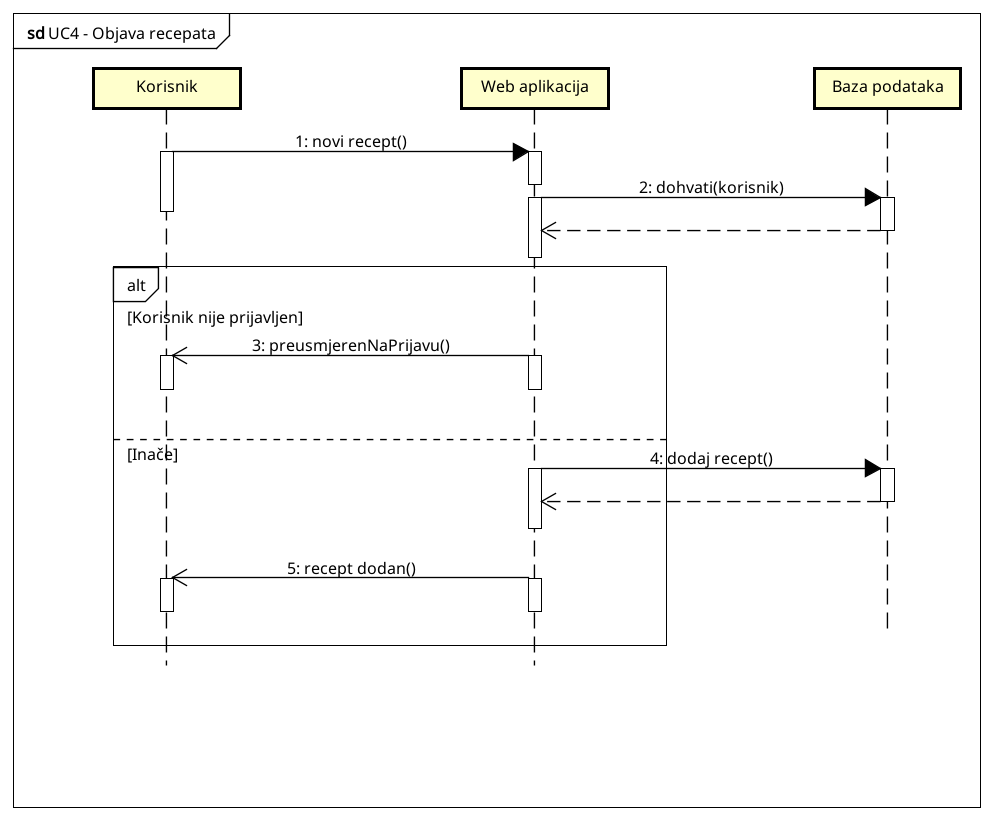
\includegraphics[scale= 0.6]{slike/sekvencijski_dijagramUC4.png}
					\centering
					\caption{Sekvencijski dijagram za UC4}
					\label{fig:Sekvencijski dijagram za UC4}
				\end{figure}
				
				\eject
				
				\noindent
				\textbf{Obrazac uporabe UC8-Videopoziv}\newline
				{Korisnik zatraži video poziv s drugim korisnikom. Ako drugi korisnik ne postoji, poziv se ne uspostavlja i o tome se obavijesti prvog korisnika. Inače se šalje zahtjev za video pozivom drugom korisniku, koji ga može odbiti ili prihvatiti. Ako odbije poziv se ne uspostavlja i o tome se obavijesti prvi korsnik. Ako prihvati uspostavi se video poziv između dva korisnika.}
				
				
				\begin{figure}[H]
					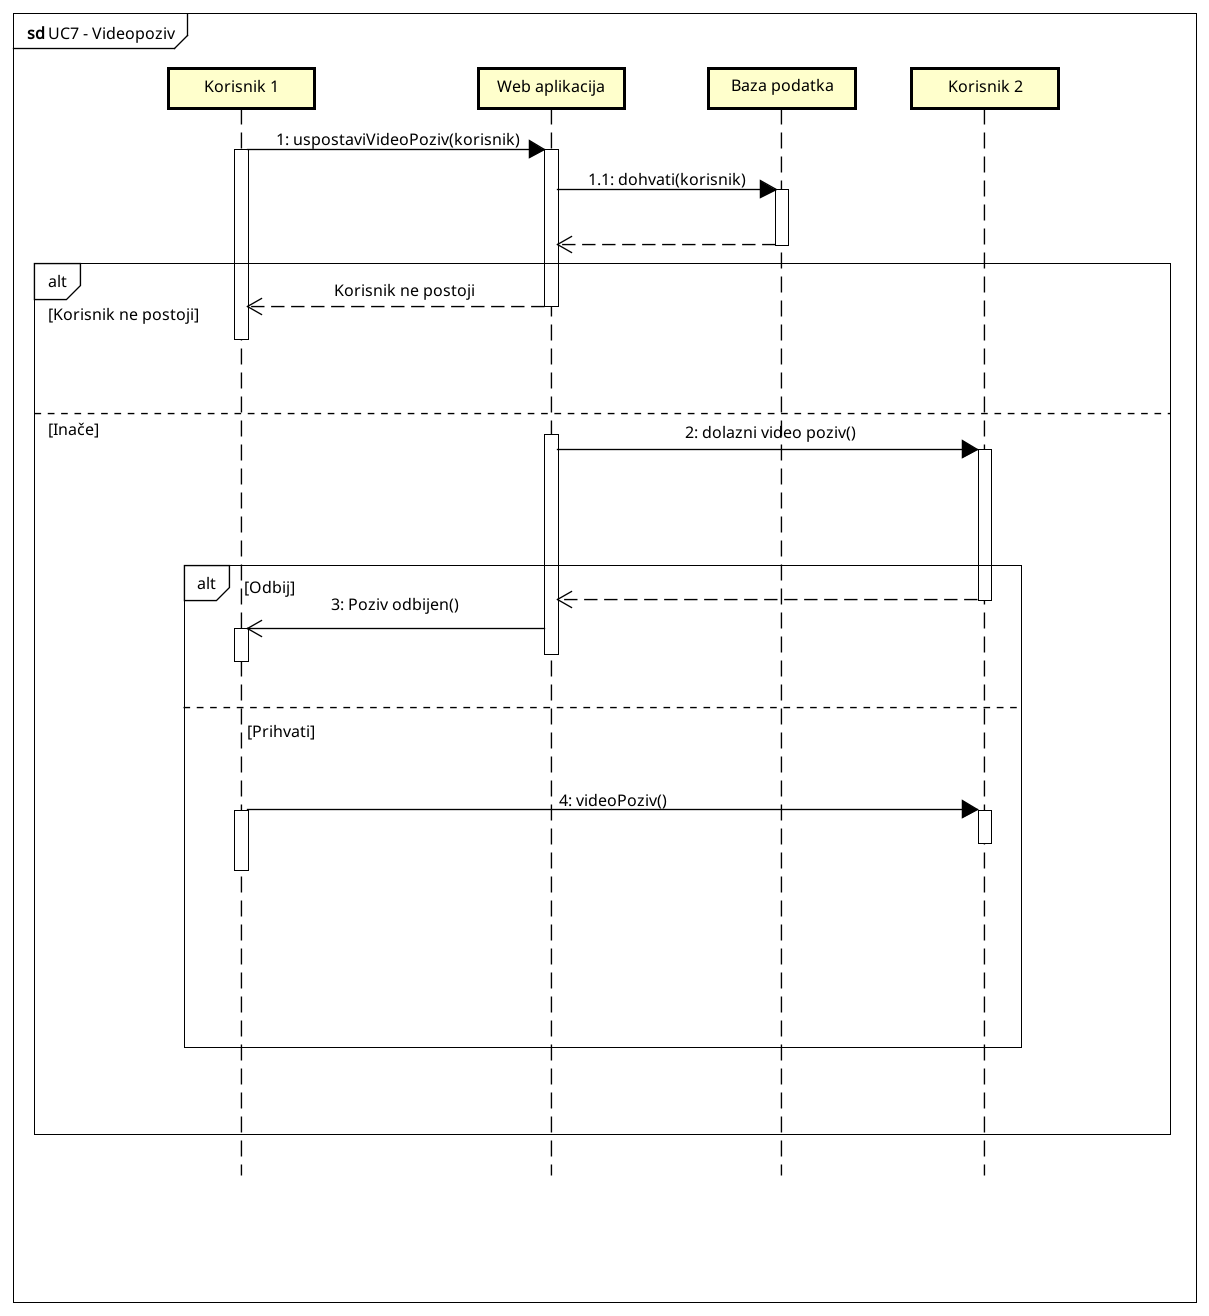
\includegraphics[scale= 0.5]{slike/sekvencijski_dijagramUC7.png}
					\centering
					\caption{Sekvencijski dijagram za UC7}
					\label{fig:Sekvencijski dijagram za UC7}
				\end{figure}
				
				\eject
				
				\section{Ostali zahtjevi}
				
				\textit{Nefunkcionalne zahtjeve koji će se navesti u nastavku teksta pojašnjavaju dodatne zahtjeve koje web aplikacija treba koristiti ili već koristi.}
				
				\begin{packed_item}
					
					\item Sustav treba biti implementiran kao web aplikacija koristeći objektno-orijentirane paradigme i norme kako bi se omogućilo ponovno korištenje dijelova koda/modula.
					\item Nepravilno korištenje web aplikacije ne smije rezultirati padom sustava.
					\item U sustavu treba biti omogućen rad i korištenje web aplikacije od strane više korisnika (cca. 50).
					\item Sustav treba omogućiti komuniciranje korisnika s ostalim korisnicima putem tekstualnog chat-a i video poziva.
					\item Sustav mora podržati dijakritičke znakove hrvatskoj jezika, dakle treba podržati hrvatsku abecedu.
					\item Hrvatski jezik je zadani jezik unutar web aplikacije.
					\item Sustav mora imati intuitivno sučelje koje neće stvarati nedoumice kod korisnika odnosno web-aplikacija treba biti jednostavna za korištenje.
					\item Konekcija s bazom podataka mora imati brz odziv. Bilo kakav pokušaj neovlaštenog pristupa informacijama u bazi podataka potrebno je spriječiti i istu adekvatno zašititi.
					\item Web aplikacija koristi proces kripitiranja lozinki za prijavu korisnika koji se tako u hash-ovima spremaju u bazu podataka.
					\item Sustav mora omogućiti korištenje određenih funkcionalnosti samo prijavljenim/registriranim korisnicima.
					\item Učitavanje početne stranice web aplikacije ne smije trajati duže od 5 sekundi.
					\item Pristup sustavu i razmjena podataka se vrši HTTPS protokolom.
					\item Pri razvoju web aplikacije koristi se React Native i Spring framework u Java programskom jeziku.
					
				\end{packed_item}
